\documentclass{beamer}
\addtobeamertemplate{navigation symbols}{}{%
\usebeamerfont{footline}%
\usebeamercolor[fg]{footline}%
\hspace{5em}%
Слайд №\insertframenumber
}
\setbeamercolor{footline}{fg=blue}
%\usetheme{Warsaw}

\usepackage[english, russian]{babel}

\usepackage{fontspec}
\setmainfont{Times New Roman}
\setsansfont{Times New Roman}
\setmonofont{Consolas}

\usepackage{sudoku}
\usepackage{tikz}
\usepackage{blkarray}
\usepackage{listings}
\lstset{basicstyle=\footnotesize\ttfamily}
\lstset{escapeinside={<@}{@>}}
\usepackage[cache=false]{minted}
\newminted{python}{fontsize=\scriptsize, linenos=false}

\graphicspath{{../images/}}

\title{Решатель судоку по изображению с камеры}
\subtitle{}
\author{А.~А.~Муравцев\inst{1}}

\institute{
\inst{1}
Высшая школа теоретической механики\\
Санкт-Петербургский Политехнический университет Петра Великого
}

\definecolor{new_green}{rgb}{0.20,0.68,0}
\begin{document}

\renewcommand*\sudokuformat[1]{\Large\sffamily#1}

\frame{\titlepage}

\begin{frame}
\frametitle{Структура проекта}
\tableofcontents
\end{frame}

\begin{frame}[fragile]
\frametitle{Структура проекта}
\begin{lstlisting}
sudoku
.
|__frontend
|  |__sudoku_app.py <@\textcolor{new_green}{(запуск графического приложения)}@>
|__lib
|  |__image_preprocess.py
|  |__sudoku_detection.py
|  |__sudoku_solver.py <@\textcolor{new_green}{(р-ль на основе рекурсивного перебора)}@>
|  |__solver_algorithm_x.py <@\textcolor{new_green}{(решатель на основе алгоритма X)}@>
|__ml_model
|  |__dataset <@\textcolor{new_green}{(датасет с изображениями напечатанных цифр)}@>
|  |__ml_train.py <@\textcolor{new_green}{(код обучения нейросети на основе dataset)}@>
|  |__printed_digit_recognition_net.h5 <@\textcolor{new_green}{(обученная нейросеть)}@>
|__tests
|  |__sudoku_pytest.py <@\textcolor{new_green}{(тесты)}@>
|__main.py <@\textcolor{new_green}{(основной файл с выводом результатов в консоль)}@>
|__exploration.py <@\textcolor{new_green}{(для исследования идей)}@>

\end{lstlisting}

\end{frame}


\section{Распознавание и обработка судоку на изображении}
\subsection{Цветное в чёрно-белое}
\begin{frame}
\frametitle{Преобразование в чёрно-белое изображение}
\begin{center}
\begin{tikzpicture}
	\node[inner sep=0pt] (to_black_white) at (0,0) {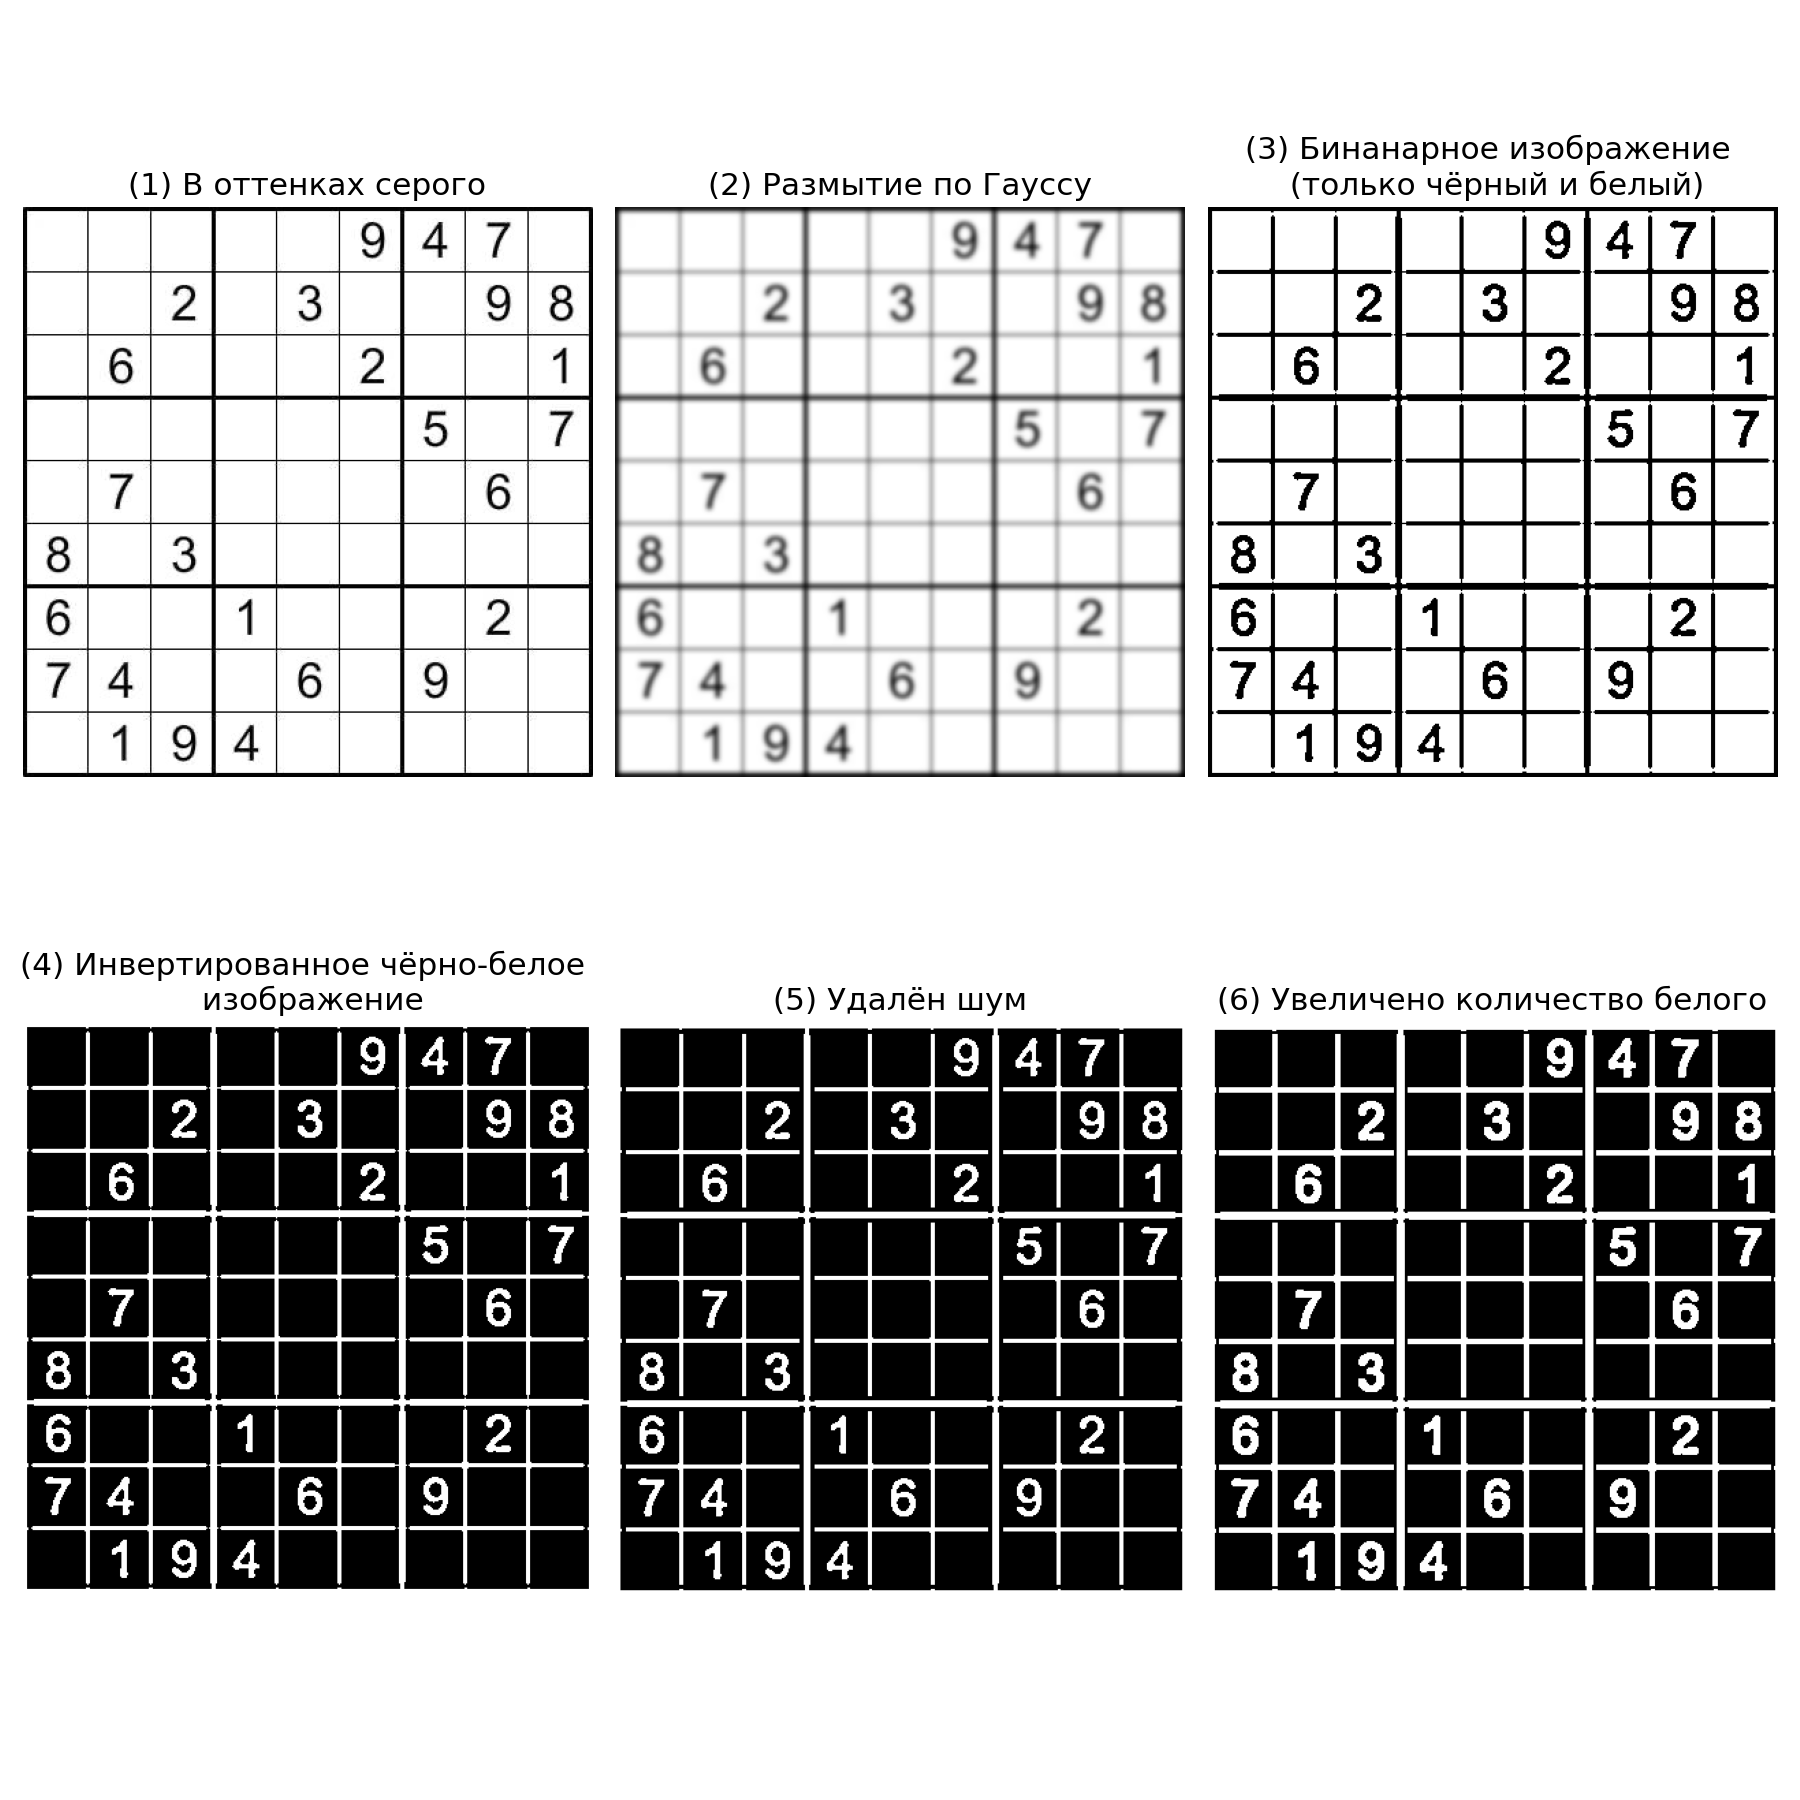
\includegraphics[width=0.7\textwidth]{to_black_white}};
\end{tikzpicture}
\end{center}

\end{frame}


\subsection{Определение местоположения поля судоку на кадре}
\begin{frame}
\frametitle{Распознавание поля судоку}

\begin{center}
\setlength\sudokusize{6cm}
\begin{sudoku-block}
| |2| | |3| |9| |7|.
| |1| | | | | | | |.
|4| |7| | | |2| |8|.
| | |5|2| | | |9| |.
| | | |1|8| |7| | |.
| |4| | | |3| | | |.
| | | | |6| | |7|1|.
| |7| | | | | | | |.
|9| |3| |2| |6| |5|.
\end{sudoku-block}
\end{center}

\end{frame}


\subsection{Разделение на ячейки}
\begin{frame}
\frametitle{Разделение на ячейки}
\end{frame}




\subsection{Распознавание цифр в ячейках с помощью обученной нейронной сети}
\begin{frame}
\frametitle{Нейросеть Keras}
\end{frame}



\section{Решатель судоку}

\subsection{Рекурсивный перебор}
\begin{frame}
\frametitle{Рекурсивный перебор}

\end{frame}




\subsection{Постановка задачи о точном покрытии}
\begin{frame}

\frametitle{Задача о точном покрытии}

Дано множество $X$ и другое множество $S$, каждый элемент которого есть подмножество множества $X$. Требуется найти такое подмножество $S^{\,*}$ множества $S$, чтобы каждый элемент из $X$ был ровно в одном элементе выбранного подмножества.\\

Пример.

Пусть $X=\{0,1,2,3,4,5,6,7,8\}$.

Пусть $S=\{A,B,C,D,E\}$, где $A=\{0,1,4,6\}$, $B=\{2,3,5\}$, $C=\{0,4,8\}$, $D=\{0,3,3,4,5,7,8\}$, $E=\{1,6,7\}$.

Тогда $S^{\,*}=\{B,C,E\}$ удовлетворяет поставленным условиям.


\end{frame}


\begin{frame}

\frametitle{Удобное представление данных задачи о точном покрытии}

$X=\{0,1,2,3,4,5,6,7,8\}$\\

$S=\{A,B,C,D,E\}$, где $A=\{0,1,4,6\}$, $B=\{2,3,5\}$, $C=\{0,4,8\}$, $D=\{0,2,3,4,5,7,8\}$, $E=\{2,6,7\}$\\
\ \\

\begin{blockarray}{cccccccccc}
 & 0 & 1 & 2 & 3 & 4 & 5 & 6 & 7 & 8 \\
\begin{block}{c(ccccccccc)}
	A & 1 & 1 & 0 & 0 & 1 & 0 & 1 & 0 & 0 \\
	\textcolor{blue}{B} & \textcolor{blue}{0} & \textcolor{blue}{0} & \textcolor{blue}{1} & \textcolor{blue}{1} & \textcolor{blue}{0} & \textcolor{blue}{1} & \textcolor{blue}{0} & \textcolor{blue}{0} & \textcolor{blue}{0} \\
	\textcolor{blue}{C} & \textcolor{blue}{1} & \textcolor{blue}{0} & \textcolor{blue}{0} & \textcolor{blue}{0} & \textcolor{blue}{1} & \textcolor{blue}{0} & \textcolor{blue}{0} & \textcolor{blue}{0} & \textcolor{blue}{1} \\
	D & 1 & 0 & 1 & 1 & 1 & 1 & 0 & 1 & 1 \\
	\textcolor{blue}{E} & \textcolor{blue}{0} & \textcolor{blue}{1} & \textcolor{blue}{0} & \textcolor{blue}{0} & \textcolor{blue}{0} & \textcolor{blue}{0} & \textcolor{blue}{1} & \textcolor{blue}{1} & \textcolor{blue}{0} \\ 
\end{block}

	
\end{blockarray}

\end{frame}



\begin{frame}

\frametitle{Судоку в терминах задачи о точном покрытии}

\hspace*{-1cm}
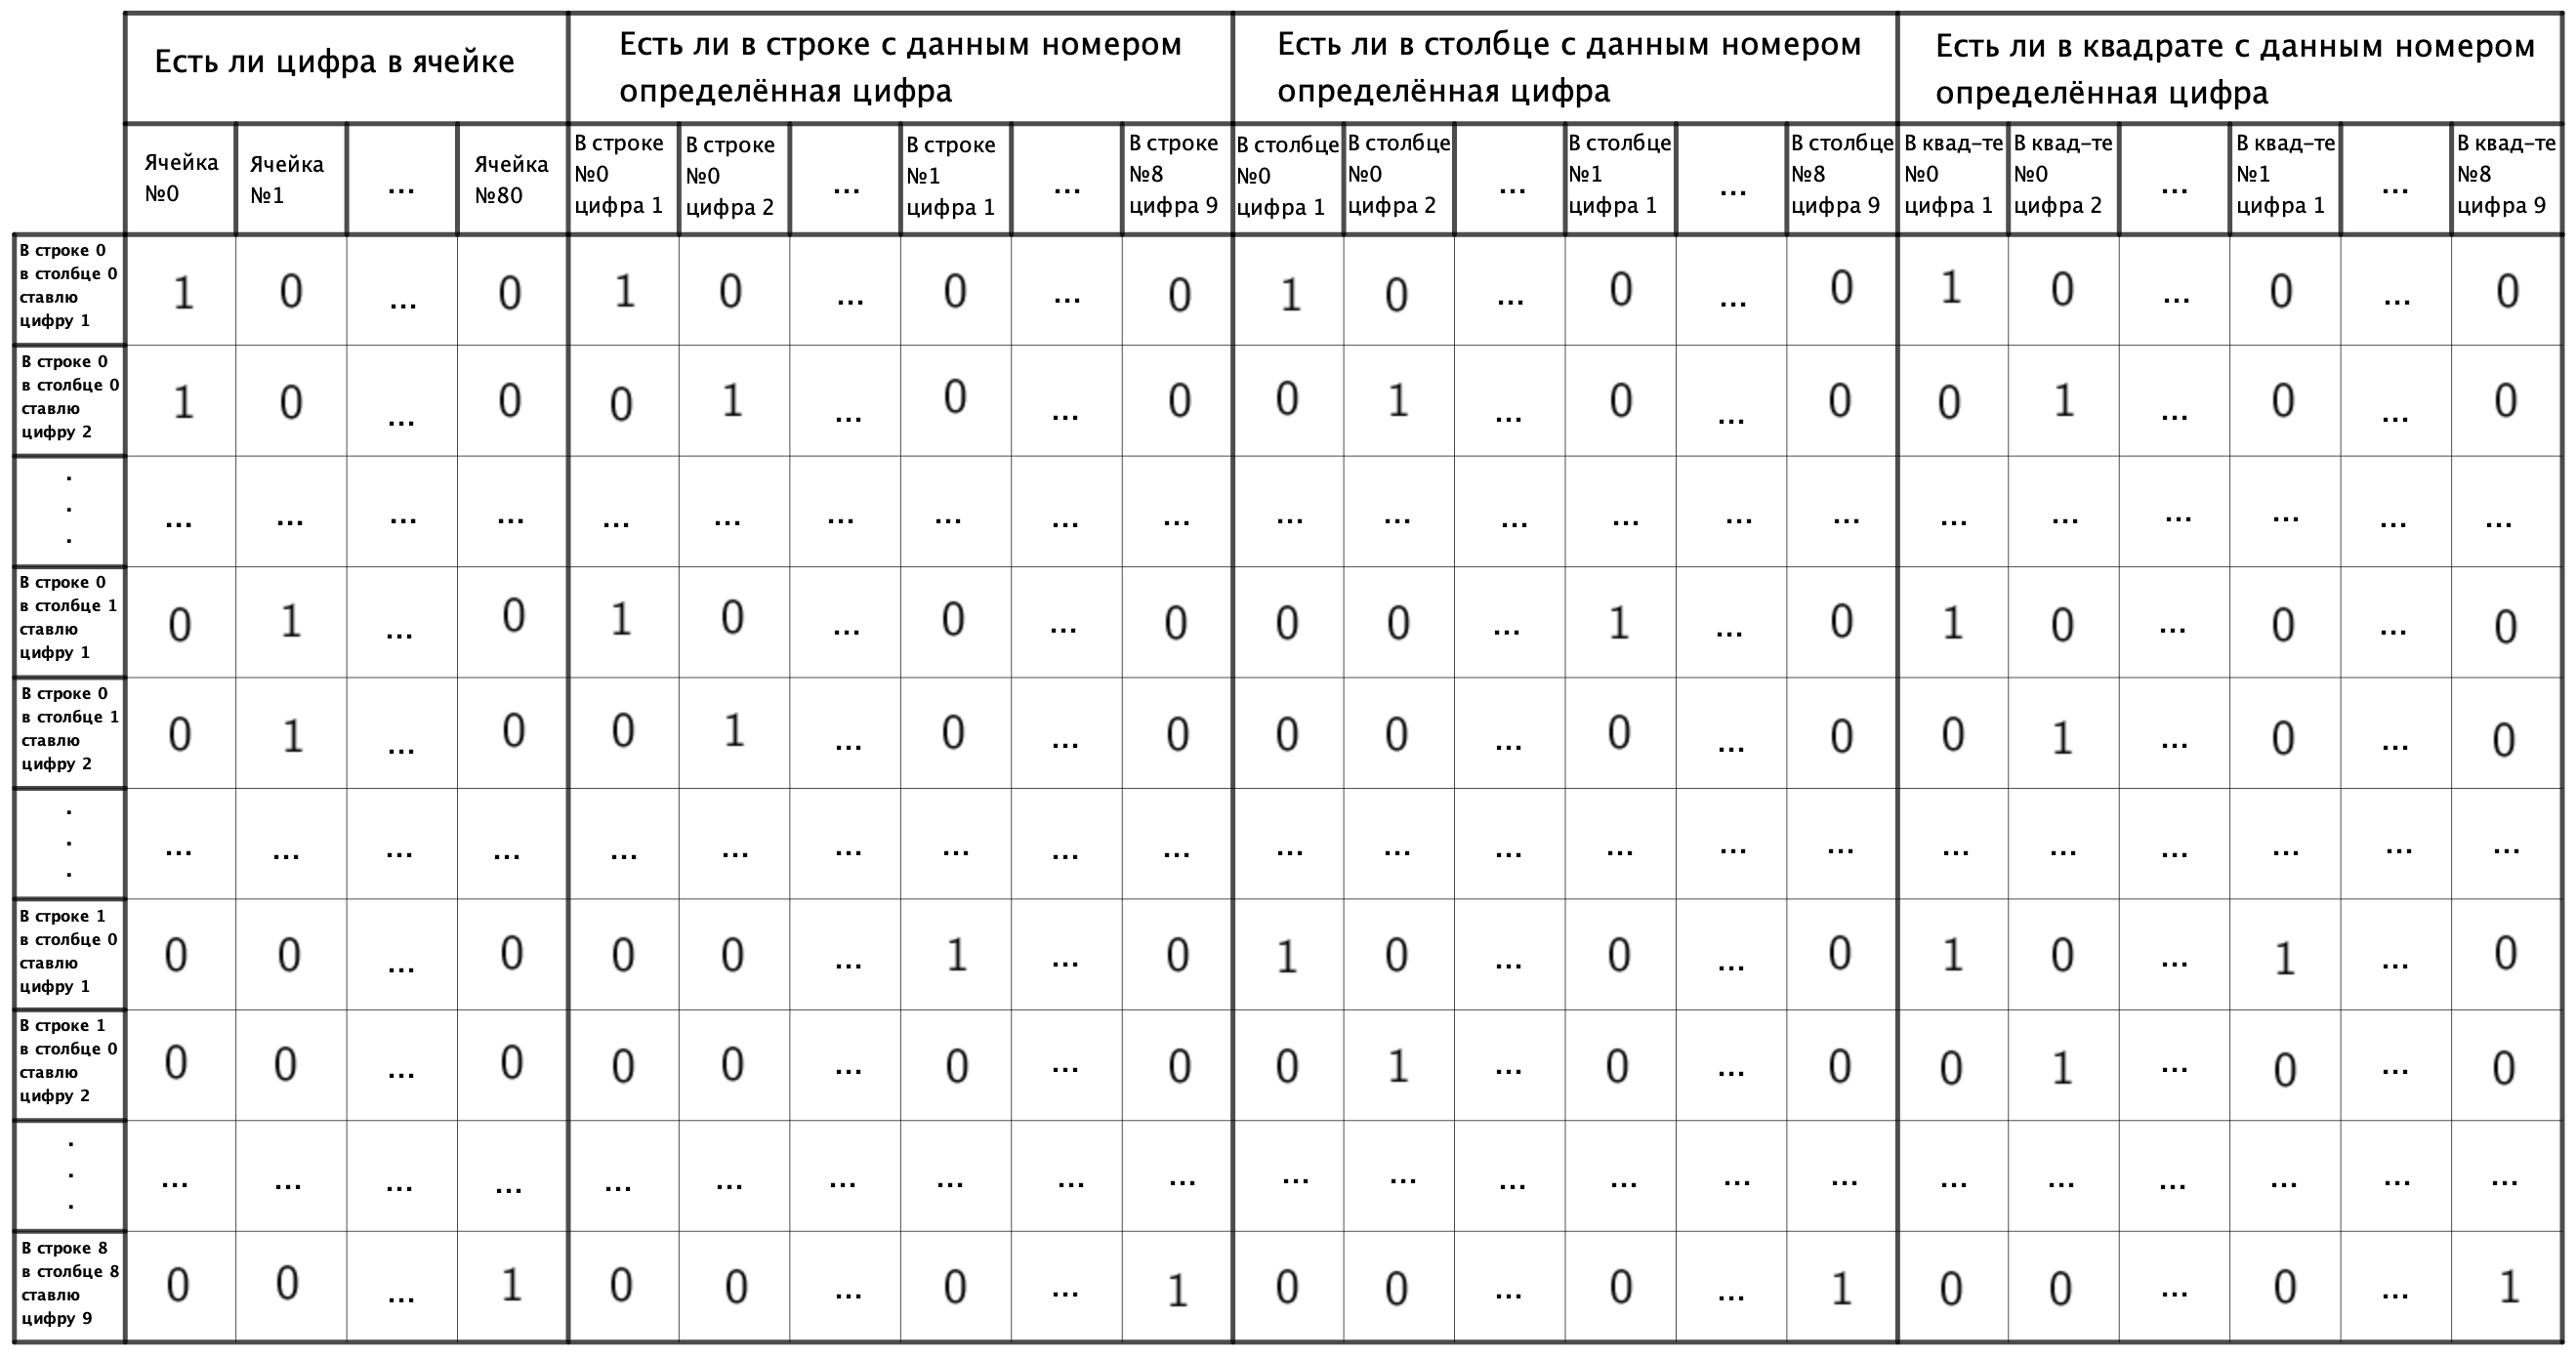
\includegraphics[width=1.15\textwidth]{SudokuToExactCoverProblem}


\end{frame}



\subsection{Алгоритм X и его реализация с помощью метода танцующих ссылок}
\begin{frame}
\frametitle{Алгоритм X}

\end{frame}



\section{Графическое приложение на PyQT}

\begin{frame}
\frametitle{Интерфейс GUI-приложения}
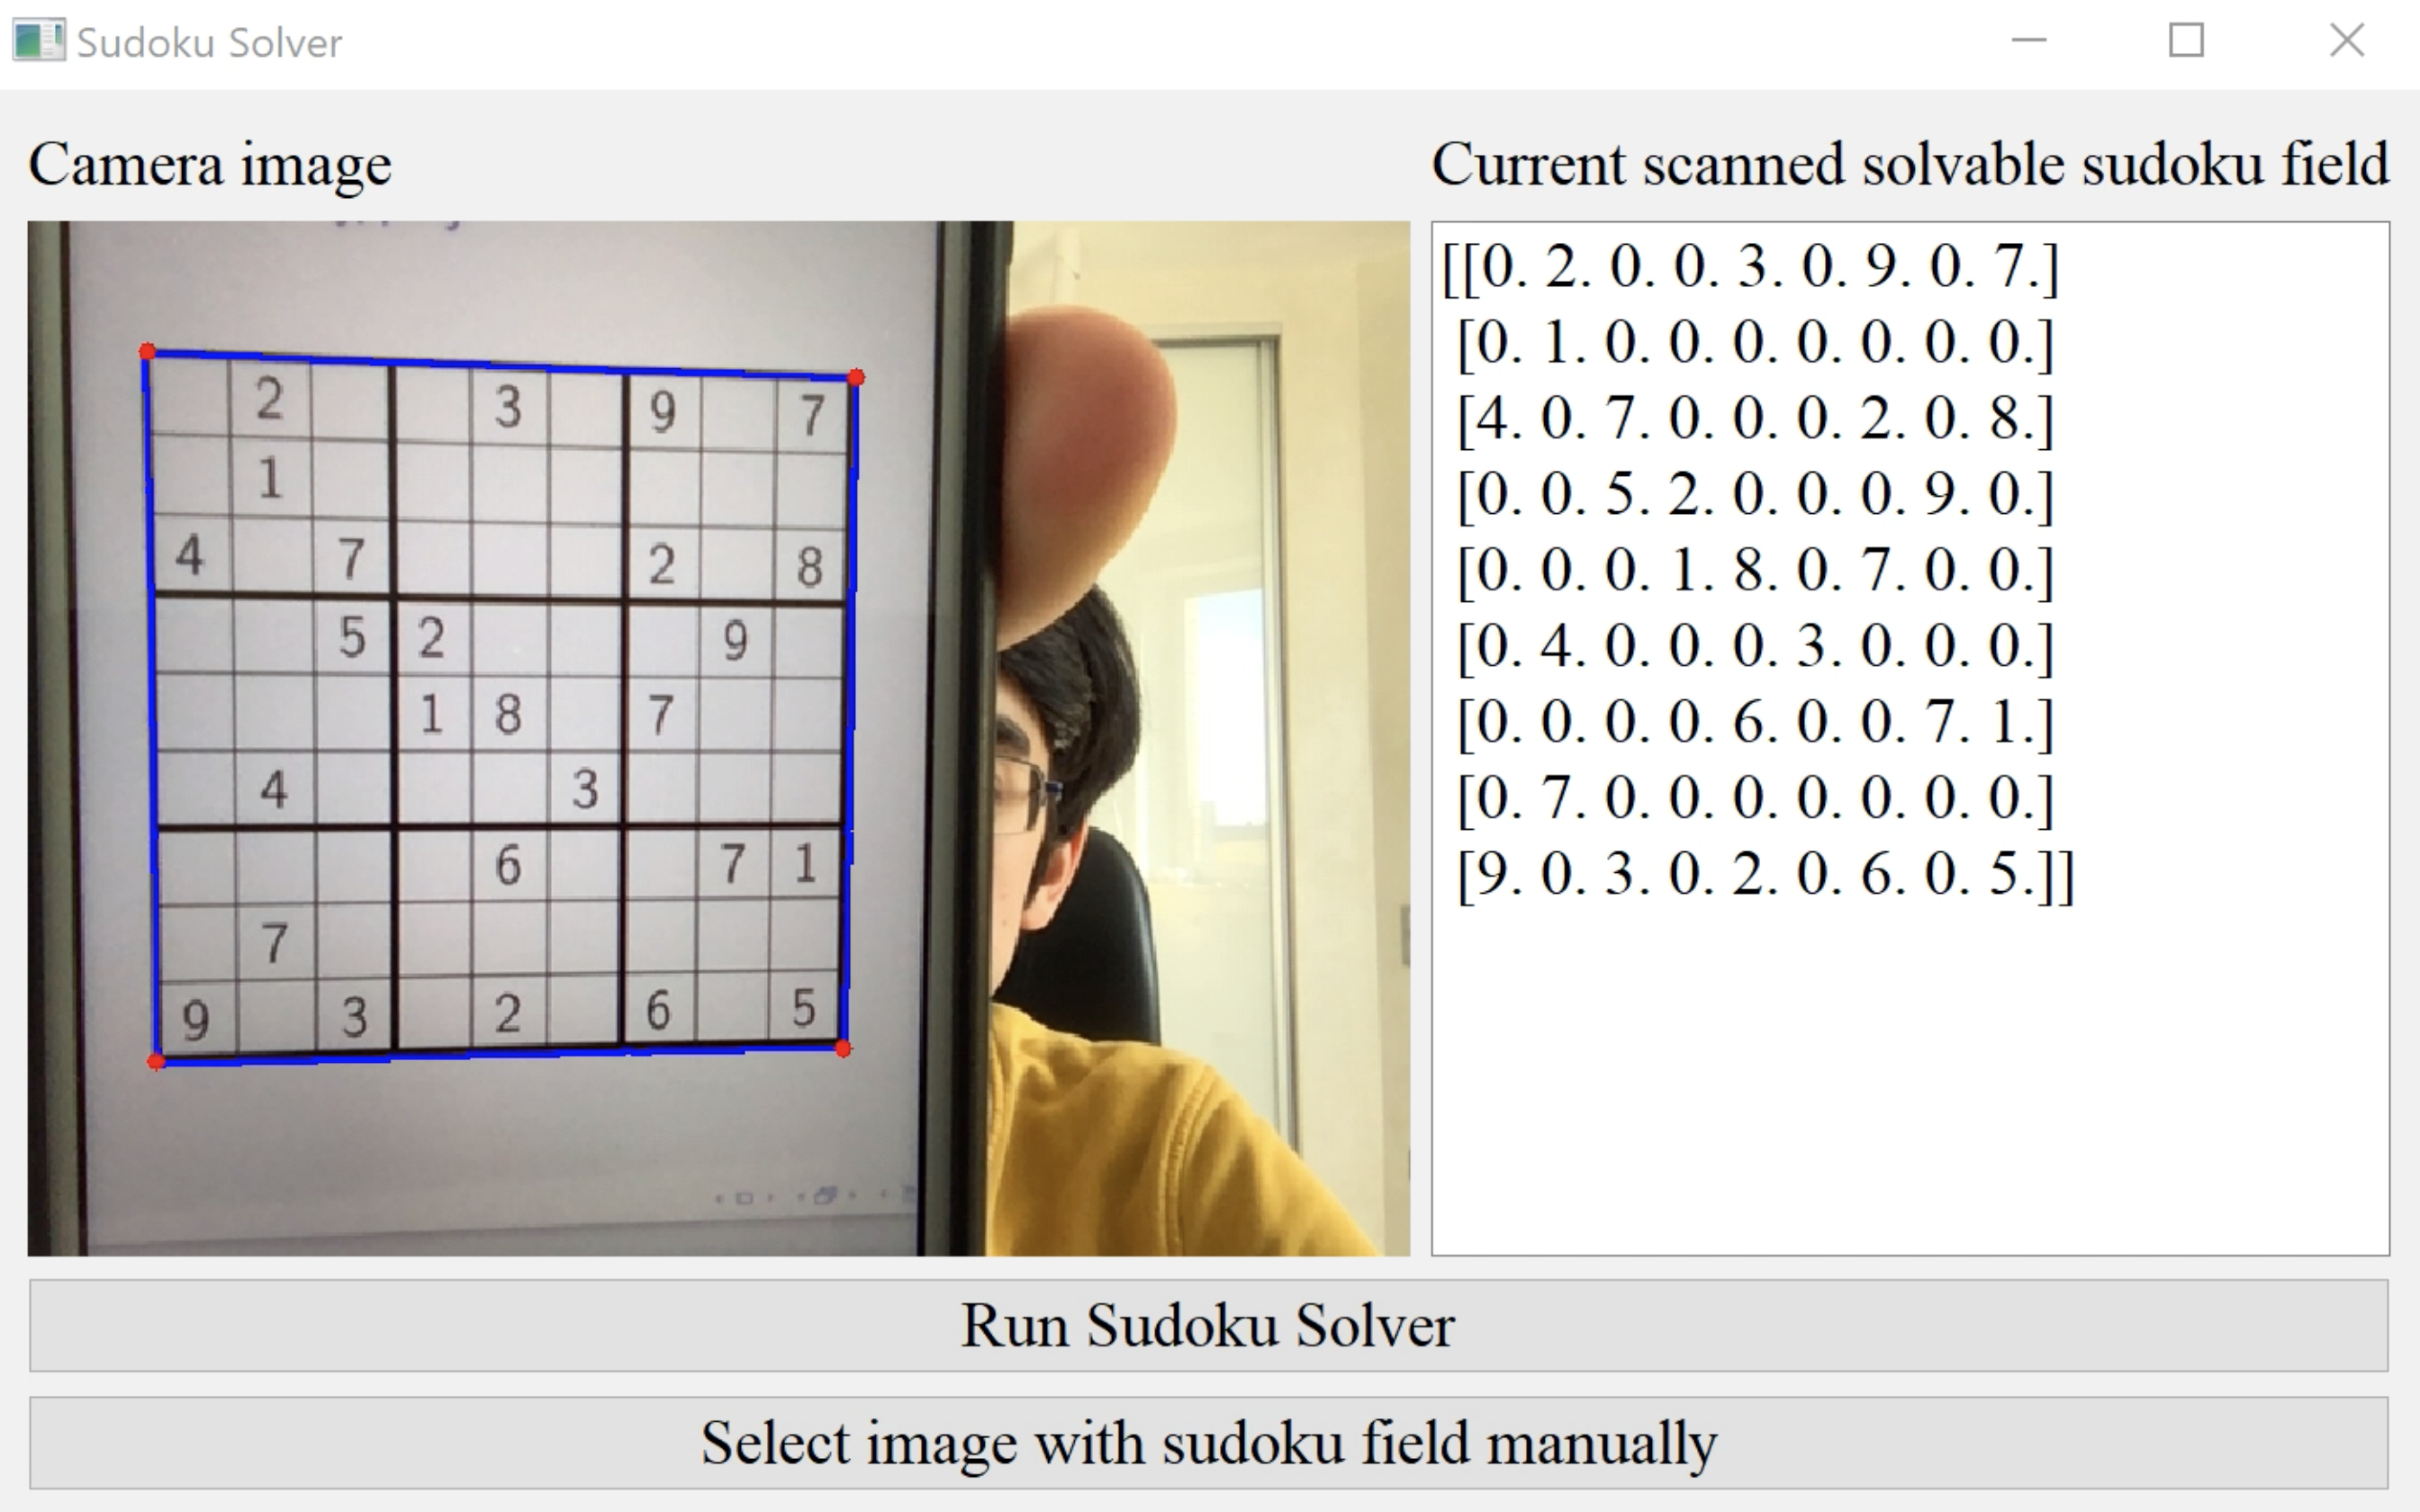
\includegraphics[width=\textwidth]{sudoku_app_in_action}
\end{frame}

\begin{frame}[fragile]
\frametitle{Слоты PyQT}

Слот преобразования openCV изображения в PyQT изображение:
\begin{pythoncode}
    @pyqtSlot(np.ndarray)
    def update_image(self, cv_img):
        """Updates the image_label with a new openCV image"""
        qt_img = self.convert_cv_to_qt(cv_img)
        self.frame_field.setPixmap(qt_img)
\end{pythoncode}
\ \\
Слот обновления текста внутри QTextEdit:
\begin{pythoncode}
    @pyqtSlot(np.ndarray)
    def update_text(self, sudoku_to_solve):
        """Updates the image_label with a new openCV image"""
        self.scanned_sudoku.setText(np.array2string(sudoku_to_solve))
\end{pythoncode}

\end{frame}


\begin{frame}[fragile]
\frametitle{Поток с результатом}
\begin{pythoncode}
class ThreadWithResult(threading.Thread):
    def __init__(self, group=None, target=None, name=None,
                 args=(), kwargs={}, *, daemon=None):
        self.result = None

        def function():
            self.result = target(*args, **kwargs)
        super().__init__(group=group, target=function,
                         name=name, daemon=daemon)
\end{pythoncode}

\end{frame}

\end{document}
